% Created 2024-05-02 Thu 16:23
% Intended LaTeX compiler: pdflatex
\documentclass[letterpaper]{article}
\usepackage[utf8]{inputenc}
\usepackage[T1]{fontenc}
\usepackage{graphicx}
\usepackage{longtable}
\usepackage{wrapfig}
\usepackage{rotating}
\usepackage[normalem]{ulem}
\usepackage{amsmath}
\usepackage{amssymb}
\usepackage{capt-of}
\usepackage{hyperref}
\usepackage{lmodern}
\usepackage{minted}
\usepackage{amsmath}
\usepackage{amsthm}
\usepackage[left=0.5in, right=0.75in, top=0.5in, bottom=0.75in]{geometry}
\usepackage{sectsty}
\usepackage[labelformat=empty]{caption}
\usepackage{parskip}
\usepackage{mdframed}
\usepackage{caption}
\sectionfont{\centering}
\usepackage{titlesec}
\usepackage{venndiagram}
\usepackage{xcolor}
\usepackage{tikz}
\usepackage{multirow}
\usepackage{listings}
\usepackage{subcaption}
\usepackage{wrapfig}
\usepackage{graphicx}
\titleformat{\section}{\centering\large\bfseries}{\thesection}{1em}{}
\titleformat{\subsection}{\centering\large\bfseries}{\thesubsection}{1em}{}
\titleformat{\subsubsection}{\normalsize\bfseries}{1pt}{1pt}{}
\theoremstyle{definition}
\newtheorem*{theorem}{Theorem}
\newtheorem*{definition}{Definition}
\newtheorem*{lemma}{Lemma}
\newtheorem*{example}{Example}
\newtheorem*{corollary}{Corollary}
\newtheorem*{remark}{Remark}
\newtheorem*{note}{Note}
\renewcommand\qedsymbol{QED}
\usepackage{hyperref}
\hypersetup{colorlinks=true, linkcolor=magenta, urlcolor=magenta}
\usepackage{listings}
\lstset{basicstyle=\ttfamily,mathescape}
\author{Hecate}
\date{\today}
\title{}
\hypersetup{
 pdfauthor={Hecate},
 pdftitle={},
 pdfkeywords={},
 pdfsubject={},
 pdfcreator={Emacs 29.3 (Org mode 9.6.15)}, 
 pdflang={English}}
\begin{document}

\begin{center}
    \large\textsc{University of California, Los Angeles} \\
    \large\textbf{Cyrus Asasi} \\
    \large\textsc{506014946}
        
    \begin{minipage}[t]{0.5\textwidth}
        \raggedright
        \textbf{ECE M146}
    \end{minipage}%
    \begin{minipage}[t]{0.5\textwidth}
        \raggedleft
        \textbf{Prof. Suhas Diggavi}
    \end{minipage}
    \centering
    \large\textbf{Homework } \\
    \large\textit{Due Saturday, May 4th, 2024 11:59pm} \textbf{via Gradescope}
\end{center}
\vspace{0.5cm}

\begin{enumerate}
\item In each of these problems, give a clear explanation for your
choice.

\begin{enumerate}
\item In the ID3 algorithm, the resulting decision tree may sometimes
be suboptimal.

\item A node in a decision tree cannot have more than two children.

\item At any point in time, the ID3 algorithms splits the data in the
decision tree by finding the feature \(X\) that minimizes the
mutual information \(I(X ; Y)\), where \(Y\) is the label.

\item You cannot use nearest neighbor classifier when there are
categorical features in your dataset. TRUE / FALSE.

\item A \$k\$-NN classifier is more likely to overfit for larger values
of \(k\).

\item Consider a \$k\$-NN with \(k=1\) and only two samples in the
training dataset. If we use an \(\ell_{2}\) distance metric, then
the classifier is equivalent to a linear classifier.

\item Training \$k\$-NN classifiers involves only saving the training
dataset into memory. TRUE / FALSE.

\item If we set \(k=N\) where \(N\) is the number of samples in the
training data, then \$k\$-NN will output the majority class among
the training samples.

\item Deep decision trees are less likely to overfit.

\item A regularized solution which minimizes \(J(\mathbf{w})+\lambda
      R(\mathbf{w})\) leads to a model with a higher empirical training
loss \(J(\mathbf{w})\). Here \(R(\mathbf{w})\) is a regularizer e.g.
\(\|w\|_{2}^{2}\).

\item You trained a binary classifier which has very high accuracy on
training data but much lower accuracy on test data. Which of the
following statements can be true? Give 1-2 lines of reasoning
along with your answer.

\begin{enumerate}
\item This is an example of underfitting.
\item The model may not have been regularized.
\item The training and test dataset are sampled from different
distributions.
\item There are too many samples in the training set hence the
model is overfitting to training set which causes poor
performance in the test set.
\end{enumerate}
\end{enumerate}

\item You get the following data set:

\begin{center}
\begin{tabular}{c|c|c||c}
\(\mathrm{V}\) & \(\mathrm{W}\) & \(\mathrm{X}\) & \(\mathrm{Y}\)\\[0pt]
\hline
0 & 0 & 0 & 0\\[0pt]
0 & 1 & 0 & 1\\[0pt]
1 & 0 & 0 & 1\\[0pt]
1 & 1 & 0 & 0\\[0pt]
1 & 1 & 1 & 0\\[0pt]
\end{tabular}
\end{center}

Your task is to build a decision tree for classifying variable \(Y\).

\begin{enumerate}
\item Write down the entire decision tree constructed by ID3. What is
the training error of this classifier.

\item Can you find a tree with smaller height than the tree returned
by ID3 in b), which also has zero training error?

\item Consider the following process: we start at the root and prune
splits for which the information gain is less than some small
number \(\epsilon\). This is called top-down pruning. What is the
decision tree returned whenever \(\epsilon=10^{-4}\)? What is the
training set error for this tree?

\item What trees do we obtain as we vary \(\epsilon>0\)?
\end{enumerate}

\item State \([\mathrm{YES} / \mathrm{NO}]\) for the following being valid
positive semi-definite kernels or not. To receive full credit, you
must provide an associated linear mapping for the \([\mathrm{YES}]\)
case, or construct a counterexample for the \([\mathrm{NO}]\) case.
No points would be awarded for answers without justification.

\begin{enumerate}
\item The function \(k: \mathbb{R} \times \mathbb{R} \rightarrow
      \mathbb{R}_{+}\) defined as \(k\left(x,
      x^{\prime}\right)=\left(x-x^{\prime}\right)^{4}\) for all \(x,
      x^{\prime} \in \mathbb{R}\). Is this a valid kernel?

\item Let \(\mathbf{x}, \mathbf{x}^{\prime} \in \mathbb{R}^{D},
      k_{0}\left(\mathbf{x}, \mathbf{x}^{\prime}\right)\) be any valid
kernel. Let $$k\left(\mathbf{x},
      \mathbf{x}^{\prime}\right)=\|\mathbf{x}\|^{2}
      K_{0}\left(\mathbf{x},
      \mathbf{x}^{\prime}\right)\left\|\mathbf{x}^{\prime}\right\|^{2}$$

Is this a valid kernel?
\end{enumerate}

\item Suppose we are looking for a maximum-margin linear classifier
through the origin, (i.e. bias \(b=0\) ) for the hard margin SVM
formulation, (i.e., no slack variables). In other words,

$$\min \frac{1}{2}\|\mathbf{w}\|^{2} \text { s.t. } y^{(i)}
   \mathbf{w}^{T} \mathbf{x}^{(i)} \geq 1, i=1, \ldots, n$$

\begin{enumerate}
\item Given a single training vector \(\mathbf{x}=(1,1)^{T} \in
      \mathbb{R}^{2}\) with label \(y=-1\), what is the \(\mathbf{w}^{*}\)
that satisfies the above constrained minimization?

\item Suppose we have two training examples,
\(\mathbf{x}^{(1)}=(1,1)^{T} \in \mathbb{R}^{2}\) and
\(\mathbf{x}^{(2)}=(1,0)^{T} \in \mathbb{R}^{2}\) with labels
\(y^{(1)}=1\) and \(y^{(2)}=-1\). What is \(\mathbf{w}^{*}\) in this
case?

\item Suppose we now allow the bias \(b\) to be non-zero. In other
words, we now adopt the hard margin SVM formulation from
lecture, where \(\mathbf{w}=\boldsymbol{\theta}_{1: d}\) are the
parameters excluding the bias:

$$\min _{\boldsymbol{\theta}} \frac{1}{2}\|\mathbf{w}\|^{2}
      \text { s.t. } y^{(i)} \boldsymbol{\theta}^{T} \mathbf{x}^{(i)}
      \geq 1, i=1, \ldots, n$$
\end{enumerate}

How would the classifier and the margin change in the previous
question? What are \(\left(\mathbf{w}^{*}, b^{*}\right)\) ? Compare
your solutions with and without bias.

\item In this problem, we ask you to compare the classification models we
have studied till now i.e., Decision trees, K-nearest neighbors,
and Logistic regression.

\textbf{Introduction}

This data was extracted from the 1994 Census bureau database by
Ronny Kohavi and Barry Becker. For computational reasons, we have
already extracted a relatively clean subset of the data for this
homework. The prediction task is to determine whether a person
makes over \(\textdollar 50\mathrm{K}\) a year.

In this problem, we ask you to complete the analysis of what sorts
of people were likely to earn more than \(\textdollar 50\mathrm{K}\)
a year. In particular, we ask you to apply the tools of machine
learning to predict which individuals are more likely to have high
income.

\textbf{Visualization}

One of the first things to do before trying any formal machine
learning technique is to dive into the data. This can include
looking for funny values in the data, looking for outliers, looking
at the range of feature values, what features seem important, etc.

Note: We have already converted all the categorical features to
numerical ones. The target column is the last one: " \(>50
   \mathrm{k} "\), where 1 and 0 indicate \(>50 \mathrm{k}\) or \(\leq 50
   \mathrm{k}\) respectively. The feature "fnlwgt" describes the number
of people the census believes the entry represents. All the other
feature names should be self-explanatory.

\textbf{Evaluation}

Now, let us use \texttt{scikit-learn} to train a \texttt{DecisionTreeClassifier},
\texttt{KNeighborsClassifier}, and \texttt{LogisticRegression} on the data.

Using the predictive capabilities of the \texttt{scikit-learn} package is
very simple. In fact, it can be carried out in three simple steps:
initializing the model, fitting it to the training data, and
predicting new values. \({ }^{3}\)

\begin{enumerate}
\item Make histograms for each feature, separating the examples by
class (e.g. income greater than \(50 \mathrm{k}\) or smaller than
or equal to \(50 \mathrm{k}\) ). This should produce fourteen
plots, one for each feature, and each plot should have two
overlapping histograms, with the color of the histogram
indicating the class. For each feature, what trends do you
observe in the data? (Please only describe the general trend. No
need for more than two sentences per feature.)

\begin{figure}[htbp]
\centering
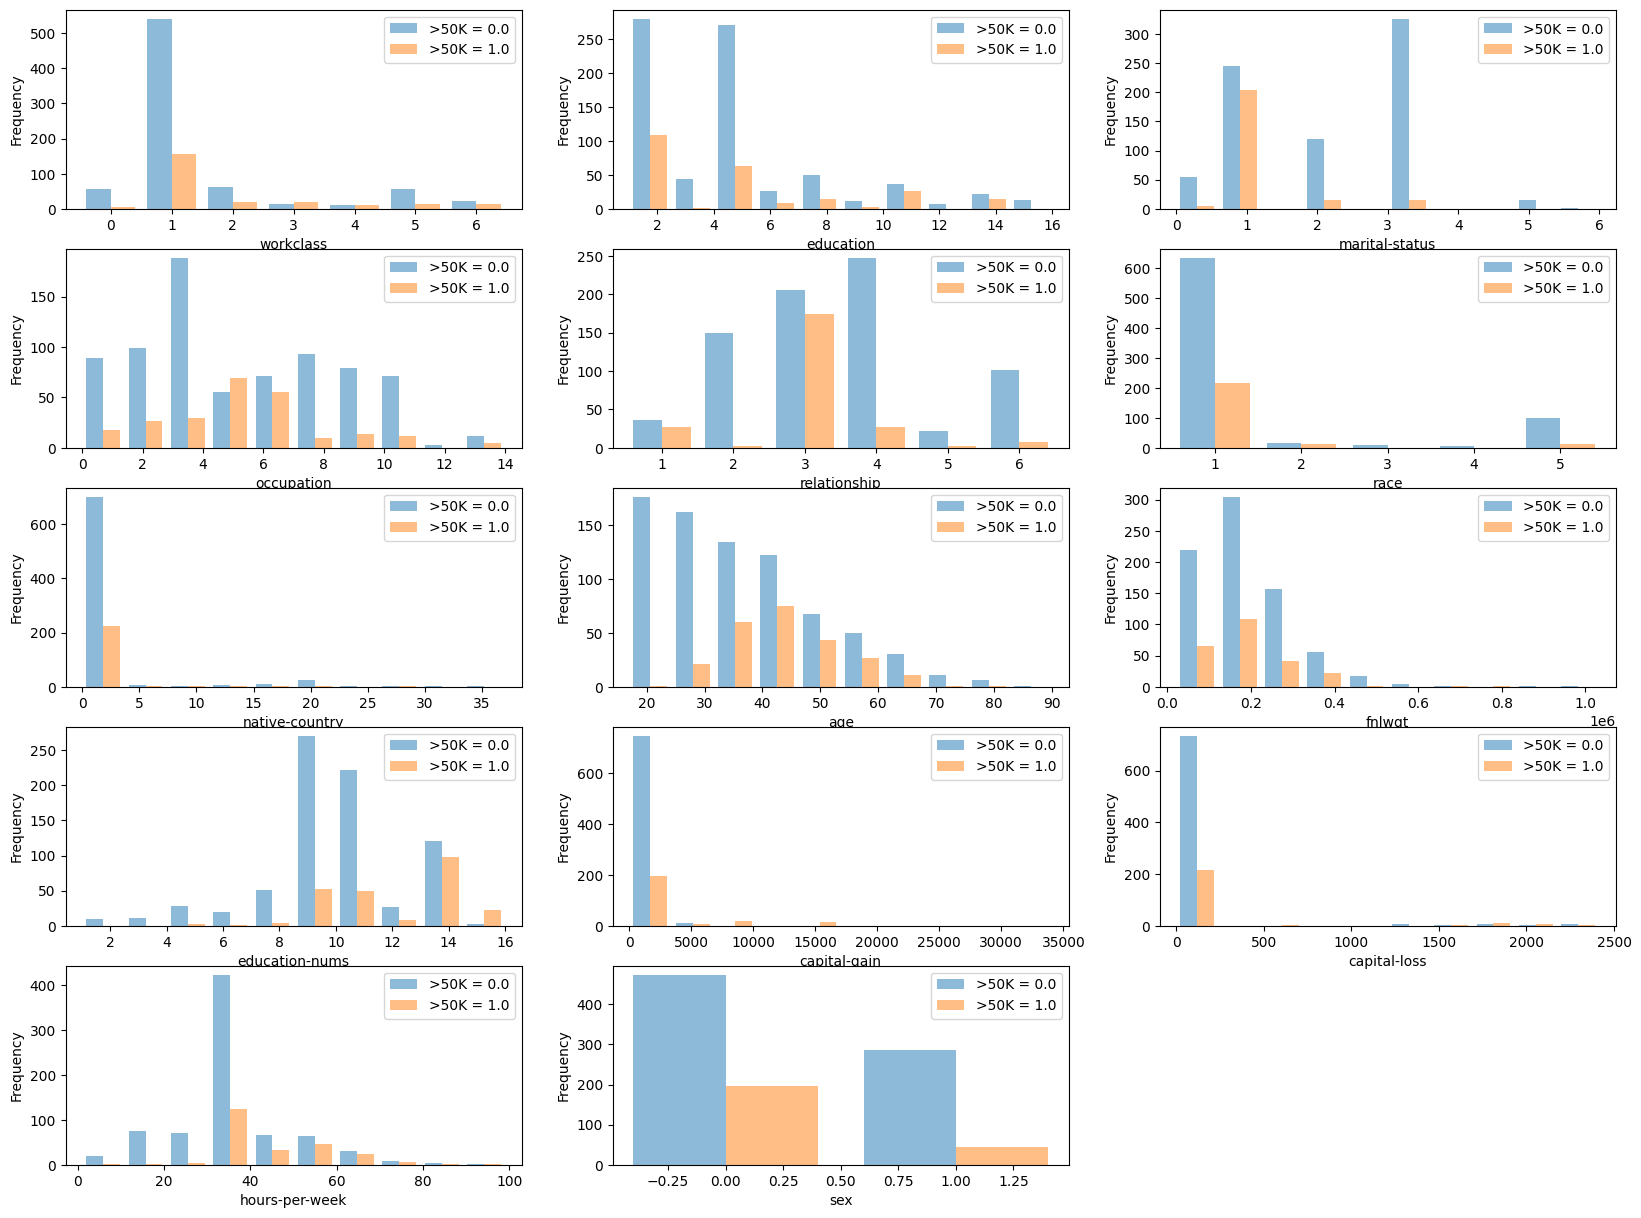
\includegraphics[width=400]{../assets/hw2_fig1.png}
\caption{Figure: Histograms of each feature separated by class}
\end{figure}

\color{teal}
\begin{enumerate}
\item For the workclass feature the histogram shows that the
majority of data points lie within workclass 1. Workclass 1
contains both the most people who make less than 50K, but
also the most people who make more than 50K in the dataset.

\item For the education feature, we can once again see most of the
data points within classes 1 through 5, which includes
individuals who's highest level of education is either a high
school or college bachelors degree.

\item Regarding the marital status feature, we can see that the
majority of our data set represents people who are in status
1 or 3, which correspond to being either divorced or
separated. However, it is interesting to note that almost all
the people in our dataset that make more than 50K a year are
divorced.

\item The occupation feature, shows how the majority of people in
our dataset are making less than 50K regardless of occupation.
The only exception is the exec-managerial occupation, in which
most of the people in our data set would make more than 50K.

\item One interesting observation about relationship status within
the dataset is that almost all of the people in our data who
make more than 50K are husbands (category 3).

\item Most of the data comes from people who identify as white.
Whites hav both the most number of people who make less than 50K,
but also the most number of people who make more than 50K.

\item Unsurprisingly for a UCI census, almost all the people who we
have data on are from the United States.

\item This feature corresponds to age, and we can see how as people
get older and reach their peak earnings throughout their
40s-50s, the number of people who are making more than 50K
increases, before decreasing again throughout retirement age.

\item TODO

\item The education number feature shows how as the number gets
higher and people get more and more educated, their earning
increases. This is shown by illustrating that most 50K+
earners are highly educated.

\item The data for capital gain shows that nearly everyone who
makes less than 50K shows low capital gain, whereas all the
people who have significant capital gain make more than 50K.

\item For capital loss, it shows that the majority of people, both
high and low earners are not experiencing capital loss
because they likely do not participate.

\item The hours-per-week feature shows clearly that people who do
not work very many hours do not earn more than 50K. Among
people who do work 40+ hours a week, we see many people
making both less than and more than 50K.

\item The sex feature shows that many more females have filled out
the census than males.
\end{enumerate}

\color{black}
\item Before trying out any classifier, it is often useful to
establish a baseline. We have implemented one simple baseline
classifier, \texttt{MajorityVoteClassifier}, that always predicts the
majority class from the training set. Read through the
\texttt{MajorityVoteClassifier} and its usage and make sure you
understand how it works.

Your goal is to implement and evaluate another baseline
classifier, \texttt{RandomClassifier}, that predicts a target class
according to the distribution of classes in the training data
set. For example, if \(85 \%\) of the examples in the training set
have \(>50 \mathrm{k}=0\) and \(15 \%\) have \(>50 \mathrm{k}=1\),
then, when applied to a test set, \texttt{RandomClassifier} should
randomly predict \(85 \%\) of the examples as \(>50 \mathrm{k}=0\)
and \(15 \%\) as \(>50 \mathrm{k}=1\).

Implement the missing portions of \texttt{RandomClassifier} according
to the provided specifications. Then train your
\texttt{RandomClassifier} on the entire training data set, and evaluate
its training error. If you implemented everything correctly, you
should have an error of \textcolor{red}{0.385} or
\textcolor{red}{0.374}, depending on an implementation detail;
both error values are correct.

\item Now that we have a baseline, train and evaluate a
\texttt{DecisionTreeClassifier} (using the class from \texttt{scikit-learn}
and referring to the documentation as needed). Make sure you
initialize your classifier with the appropriate parameters; in
particular, use the 'entropy' criterion discussed in class. What
is the training error of this classifier?

\item Similar to the previous question, train and evaluate a
\texttt{KNeighborsClassifier} (using the class from \texttt{scikit-learn} and
referring to the documentation as needed). Use \(k=3,5\) and 7 as
the number of neighbors and report the training error of this
classifier respectively.

\item Similar to the previous question, train and evaluate a
\texttt{LogisticRegression} (using the class from \texttt{scikit-learn} and
referring to the documentation as needed). Use \(\lambda=0.1,1\)
and 10 as the regularization hyperparameter and report the
training error of this classifier respectively. Make sure you
initialize your classifier with the appropriate parameters;
\texttt{random\_state=0} and \texttt{max\_iter=1000}. (Hint: function argument
\(\mathrm{C}\) is the inverse of regularization strength,
therefore \(\mathrm{C}=1 / \lambda\).)

\item So far, we have looked only at training error, but as we learned
in class, training error is a poor metric for evaluating
classifiers. Let us use cross-validation instead.

Implement the missing portions of \texttt{error(...)} according to the
provided specifications. You may find it helpful to use
\texttt{StratifiedShuffleSplit(...)} from \texttt{scikit-learn}. To ensure
that we always get the same splits across different runs (and
thus can compare the classifier results), set the random\textsubscript{state}
parameter to be the same (e.g., 0).

Next, use your \texttt{error(...)} function to evaluate the training
error and (cross-validation) validation error and validation
micro averaged F1 (if you don't know what is F1 click
\href{https://scikit-learn.org/stable/modules/generated/sklearn.metrics.f1_score.html?highlight=f1%20score#sklearn.metrics.f1_score}{here})
Score of the \texttt{RandomClassifier}, \texttt{DecisionTreeClassifier},
\texttt{KNeighborsClassifier}, and \texttt{LogisticRegression} models (for the
\texttt{DecisionTreeClassifier}, use 'entropy' criterion, for the \\[0pt]
\texttt{KNeighborsClassifier}, use \(k=5\), for the \texttt{LogisticRegression},
use \(\lambda=1\), \texttt{random\_state = 0} and \texttt{max\_iter = 1000} ). To
do this, generate a random \(85 / 15\) split of the training data,
train each model on the \(85 \%\) fraction, evaluate the error on
both the \(85 \%\) and the \(15 \%\) fraction, and repeat this 100
times to get an average result. What are the average training
error, validation error, and validation F1 score of each of your
classifiers on the \texttt{adult\_subsample} data set?

\item One way to find out the best value of \(k\) for
\texttt{KNeighborsClassifier} is \(n\text{-fold}\) cross validation. Find
out the best value of \(k\) using 5 -fold cross validation. You
may find the \texttt{cross\_val\_score(...)} from \texttt{scikit-learn} helpful.
Run 5-fold cross validation for all odd numbers ranging from 1
to 50 as the number of neighbors. Then plot the validation score
against the number of neighbors, \(k\). Include this plot in your
writeup, and provide a 12 sentence description of your
observations. What is the best value of \(k\) and what is the
corresponding score?

\item One problem with decision trees is that they can \emph{overfit} to
training data, yielding complex classifiers that do not
generalize well to new data. Let us see whether this is the case
for the \texttt{adult\_subsample} data.

One way to prevent decision trees from overfitting is to limit
their depth. Repeat your crossvalidation experiments but for
increasing depth limits, specifically, \(1,2, \ldots, 20\). Then
plot the average training error and validation error against the
depth limit. Include this plot in your writeup, making sure to
label all axes and include a legend for your classifiers. What
is the best depth limit to use for this data? Do you see
overfitting? Justify your answers using the plot.
\end{enumerate}
\end{enumerate}
\end{document}
